\hypertarget{_lgm___quad_pack_8c}{
\section{/home/mgh/LanlGeoMag/libLanlGeoMag/Lgm\_\-QuadPack.c File Reference}
\label{_lgm___quad_pack_8c}\index{/home/mgh/LanlGeoMag/libLanlGeoMag/Lgm\_\-QuadPack.c@{/home/mgh/LanlGeoMag/libLanlGeoMag/Lgm\_\-QuadPack.c}}
}
{\tt \#include \char`\"{}Lgm/Lgm\_\-QuadPack.h\char`\"{}}\par


Include dependency graph for Lgm\_\-QuadPack.c:\nopagebreak
\begin{figure}[H]
\begin{center}
\leavevmode
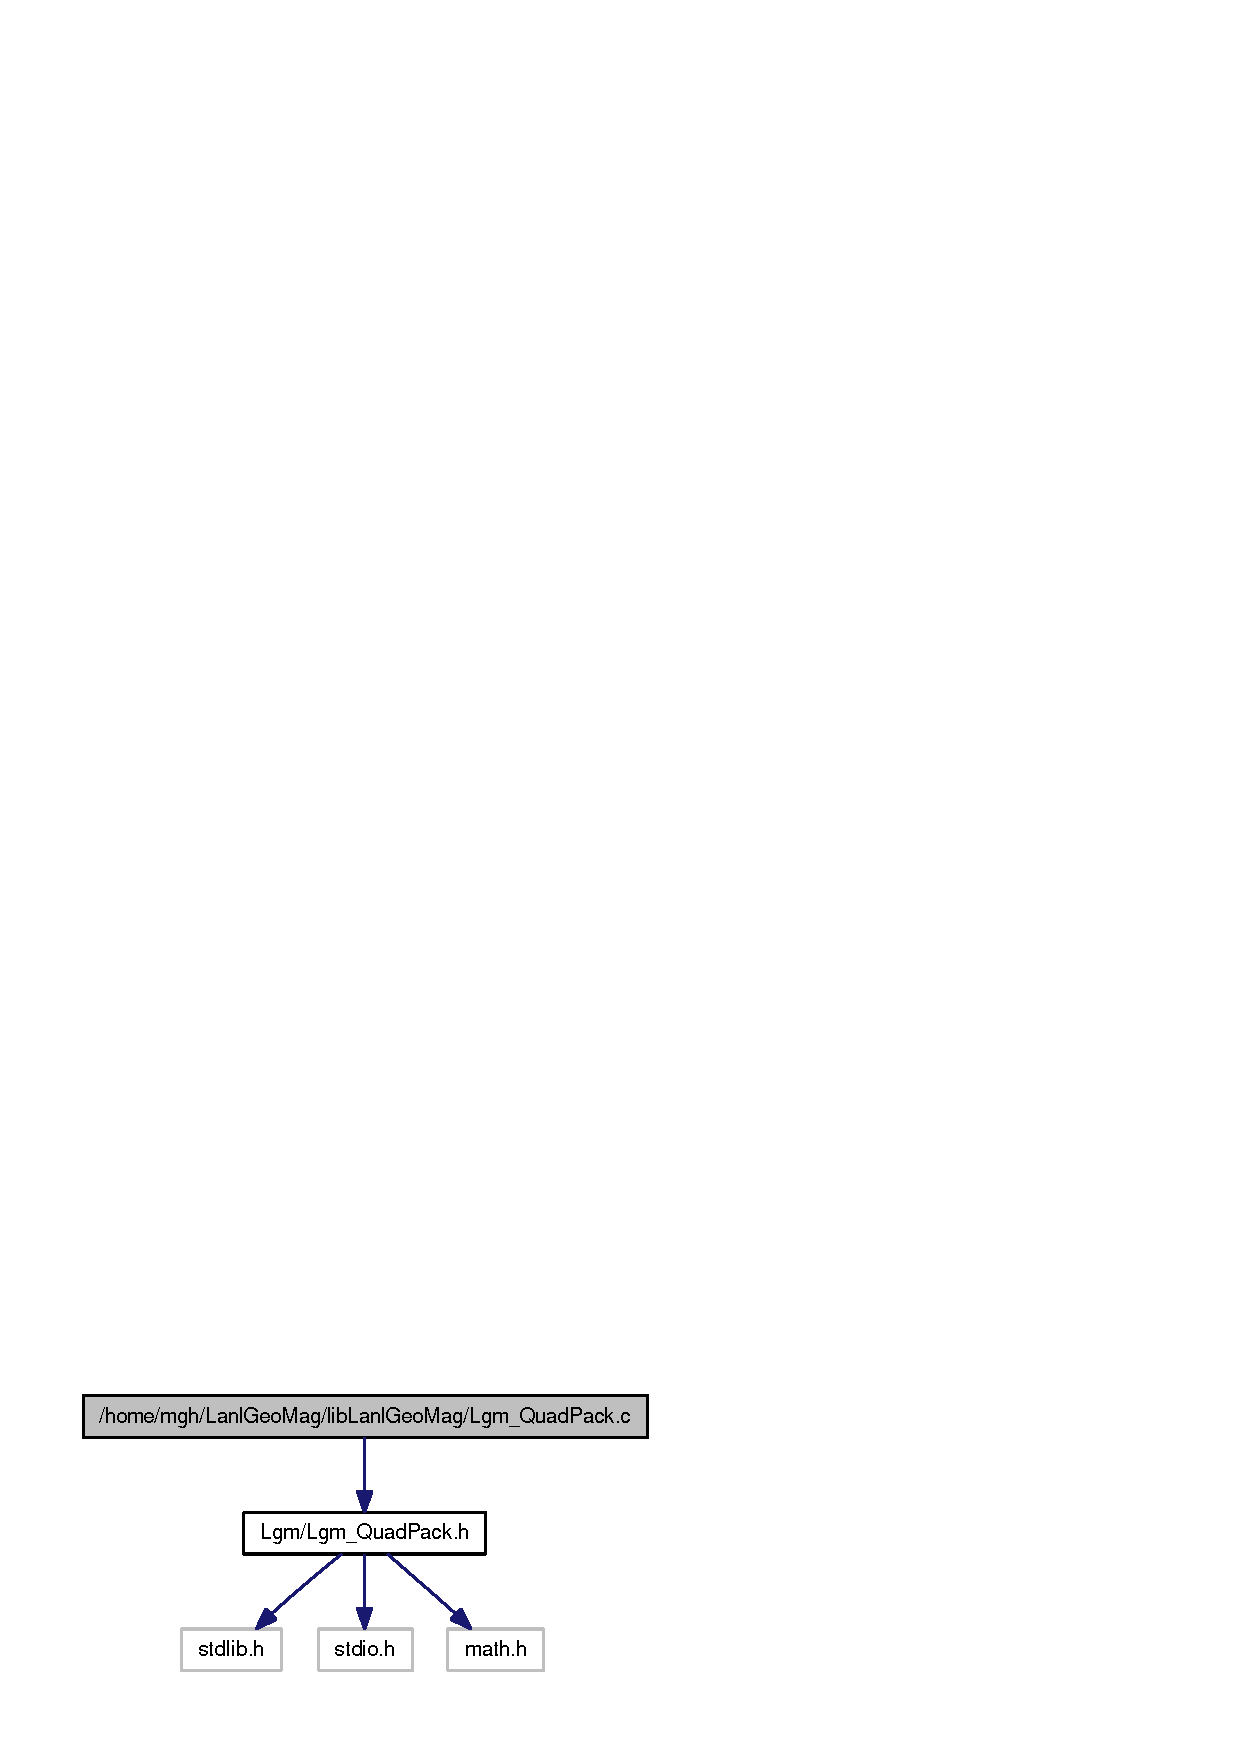
\includegraphics[width=157pt]{_lgm___quad_pack_8c__incl}
\end{center}
\end{figure}
\subsection*{Functions}
\begin{CompactItemize}
\item 
int \hyperlink{_lgm___quad_pack_8c_5dd348ebbe6031e619161d72806d443f}{dqags} (double $\ast$f, \hyperlink{_lgm___quad_pack_8h_01be5a7db8d2fc2ba26ce793d73b6472}{\_\-qpInfo} $\ast$qpInfo, double a, double b, double epsabs, double epsrel, double $\ast$result, double $\ast$abserr, int $\ast$neval, int $\ast$ier, int limit, int lenw, int $\ast$last, int $\ast$iwork, double $\ast$work)
\item 
int \hyperlink{_lgm___quad_pack_8c_8305957e8651fd6d18b1dbf6fa41e567}{dqagse} (double $\ast$f, \hyperlink{_lgm___quad_pack_8h_01be5a7db8d2fc2ba26ce793d73b6472}{\_\-qpInfo} $\ast$qpInfo, double a, double b, double epsabs, double epsrel, int limit, double $\ast$result, double $\ast$abserr, int $\ast$neval, int $\ast$ier, double $\ast$alist, double $\ast$blist, double $\ast$rlist, double $\ast$elist, int $\ast$iord, int $\ast$last)
\item 
int \hyperlink{_lgm___quad_pack_8c_cf4d898607ec70526db76c862ba787c5}{dqelg} (int n, double epstab\mbox{[}$\,$\mbox{]}, double $\ast$result, double $\ast$abserr, double res3la\mbox{[}$\,$\mbox{]}, int $\ast$nres)
\item 
int \hyperlink{_lgm___quad_pack_8c_ec57c5f0bf1379097d6e1075f3dc39c6}{dqk21} (double $\ast$f, \hyperlink{_lgm___quad_pack_8h_01be5a7db8d2fc2ba26ce793d73b6472}{\_\-qpInfo} $\ast$qpInfo, double a, double b, double $\ast$result, double $\ast$abserr, double $\ast$resabs, double $\ast$resasc)
\item 
int \hyperlink{_lgm___quad_pack_8c_2df6dbeadd2fead8bc01b016ddeff2ab}{dqpsrt} (int limit, int last, int $\ast$maxerr, double $\ast$ermax, double elist\mbox{[}$\,$\mbox{]}, int iord\mbox{[}$\,$\mbox{]}, int $\ast$nrmax)
\item 
double \hyperlink{_lgm___quad_pack_8c_8a6a37ed72bdfd824c7b178284142ad4}{d1mach} (int i)
\end{CompactItemize}


\subsection{Function Documentation}
\hypertarget{_lgm___quad_pack_8c_5dd348ebbe6031e619161d72806d443f}{
\index{Lgm\_\-QuadPack.c@{Lgm\_\-QuadPack.c}!dqags@{dqags}}
\index{dqags@{dqags}!Lgm_QuadPack.c@{Lgm\_\-QuadPack.c}}
\subsubsection[{dqags}]{\setlength{\rightskip}{0pt plus 5cm}int dqags (double  $\ast$ {\em f}, \/  {\bf \_\-qpInfo} $\ast$ {\em qpInfo}, \/  double {\em a}, \/  double {\em b}, \/  double {\em epsabs}, \/  double {\em epsrel}, \/  double  $\ast$ {\em result}, \/  double  $\ast$ {\em abserr}, \/  int     $\ast$ {\em neval}, \/  int     $\ast$ {\em ier}, \/  int {\em limit}, \/  int {\em lenw}, \/  int	$\ast$ {\em last}, \/  int	$\ast$ {\em iwork}, \/  double	$\ast$ {\em work})}}
\label{_lgm___quad_pack_8c_5dd348ebbe6031e619161d72806d443f}




Definition at line 6 of file Lgm\_\-QuadPack.c.

Here is the call graph for this function:\nopagebreak
\begin{figure}[H]
\begin{center}
\leavevmode
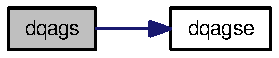
\includegraphics[width=85pt]{_lgm___quad_pack_8c_5dd348ebbe6031e619161d72806d443f_cgraph}
\end{center}
\end{figure}
\hypertarget{_lgm___quad_pack_8c_8305957e8651fd6d18b1dbf6fa41e567}{
\index{Lgm\_\-QuadPack.c@{Lgm\_\-QuadPack.c}!dqagse@{dqagse}}
\index{dqagse@{dqagse}!Lgm_QuadPack.c@{Lgm\_\-QuadPack.c}}
\subsubsection[{dqagse}]{\setlength{\rightskip}{0pt plus 5cm}int dqagse (double  $\ast$ {\em f}, \/  {\bf \_\-qpInfo} $\ast$ {\em qpInfo}, \/  double {\em a}, \/  double {\em b}, \/  double {\em epsabs}, \/  double {\em epsrel}, \/  int {\em limit}, \/  double  $\ast$ {\em result}, \/  double  $\ast$ {\em abserr}, \/  int     $\ast$ {\em neval}, \/  int     $\ast$ {\em ier}, \/  double   $\ast$ {\em alist}, \/  double   $\ast$ {\em blist}, \/  double   $\ast$ {\em rlist}, \/  double   $\ast$ {\em elist}, \/  int	 $\ast$ {\em iord}, \/  int	$\ast$ {\em last})}}
\label{_lgm___quad_pack_8c_8305957e8651fd6d18b1dbf6fa41e567}




Definition at line 252 of file Lgm\_\-QuadPack.c.

Here is the call graph for this function:\nopagebreak
\begin{figure}[H]
\begin{center}
\leavevmode
\includegraphics[width=130pt]{_lgm___quad_pack_8c_8305957e8651fd6d18b1dbf6fa41e567_cgraph}
\end{center}
\end{figure}
\hypertarget{_lgm___quad_pack_8c_cf4d898607ec70526db76c862ba787c5}{
\index{Lgm\_\-QuadPack.c@{Lgm\_\-QuadPack.c}!dqelg@{dqelg}}
\index{dqelg@{dqelg}!Lgm_QuadPack.c@{Lgm\_\-QuadPack.c}}
\subsubsection[{dqelg}]{\setlength{\rightskip}{0pt plus 5cm}int dqelg (int {\em n}, \/  double {\em epstab}\mbox{[}$\,$\mbox{]}, \/  double $\ast$ {\em result}, \/  double $\ast$ {\em abserr}, \/  double {\em res3la}\mbox{[}$\,$\mbox{]}, \/  int $\ast$ {\em nres})}}
\label{_lgm___quad_pack_8c_cf4d898607ec70526db76c862ba787c5}




Definition at line 868 of file Lgm\_\-QuadPack.c.

Here is the call graph for this function:\nopagebreak
\begin{figure}[H]
\begin{center}
\leavevmode
\includegraphics[width=86pt]{_lgm___quad_pack_8c_cf4d898607ec70526db76c862ba787c5_cgraph}
\end{center}
\end{figure}


Here is the caller graph for this function:\nopagebreak
\begin{figure}[H]
\begin{center}
\leavevmode
\includegraphics[width=84pt]{_lgm___quad_pack_8c_cf4d898607ec70526db76c862ba787c5_icgraph}
\end{center}
\end{figure}
\hypertarget{_lgm___quad_pack_8c_ec57c5f0bf1379097d6e1075f3dc39c6}{
\index{Lgm\_\-QuadPack.c@{Lgm\_\-QuadPack.c}!dqk21@{dqk21}}
\index{dqk21@{dqk21}!Lgm_QuadPack.c@{Lgm\_\-QuadPack.c}}
\subsubsection[{dqk21}]{\setlength{\rightskip}{0pt plus 5cm}int dqk21 (double  $\ast$ {\em f}, \/  {\bf \_\-qpInfo} $\ast$ {\em qpInfo}, \/  double {\em a}, \/  double {\em b}, \/  double  $\ast$ {\em result}, \/  double  $\ast$ {\em abserr}, \/  double  $\ast$ {\em resabs}, \/  double  $\ast$ {\em resasc})}}
\label{_lgm___quad_pack_8c_ec57c5f0bf1379097d6e1075f3dc39c6}




Definition at line 1130 of file Lgm\_\-QuadPack.c.

Here is the call graph for this function:\nopagebreak
\begin{figure}[H]
\begin{center}
\leavevmode
\includegraphics[width=87pt]{_lgm___quad_pack_8c_ec57c5f0bf1379097d6e1075f3dc39c6_cgraph}
\end{center}
\end{figure}
\hypertarget{_lgm___quad_pack_8c_2df6dbeadd2fead8bc01b016ddeff2ab}{
\index{Lgm\_\-QuadPack.c@{Lgm\_\-QuadPack.c}!dqpsrt@{dqpsrt}}
\index{dqpsrt@{dqpsrt}!Lgm_QuadPack.c@{Lgm\_\-QuadPack.c}}
\subsubsection[{dqpsrt}]{\setlength{\rightskip}{0pt plus 5cm}int dqpsrt (int {\em limit}, \/  int {\em last}, \/  int $\ast$ {\em maxerr}, \/  double $\ast$ {\em ermax}, \/  double {\em elist}\mbox{[}$\,$\mbox{]}, \/  int {\em iord}\mbox{[}$\,$\mbox{]}, \/  int $\ast$ {\em nrmax})}}
\label{_lgm___quad_pack_8c_2df6dbeadd2fead8bc01b016ddeff2ab}




Definition at line 1375 of file Lgm\_\-QuadPack.c.

Here is the caller graph for this function:\nopagebreak
\begin{figure}[H]
\begin{center}
\leavevmode
\includegraphics[width=86pt]{_lgm___quad_pack_8c_2df6dbeadd2fead8bc01b016ddeff2ab_icgraph}
\end{center}
\end{figure}
\hypertarget{_lgm___quad_pack_8c_8a6a37ed72bdfd824c7b178284142ad4}{
\index{Lgm\_\-QuadPack.c@{Lgm\_\-QuadPack.c}!d1mach@{d1mach}}
\index{d1mach@{d1mach}!Lgm_QuadPack.c@{Lgm\_\-QuadPack.c}}
\subsubsection[{d1mach}]{\setlength{\rightskip}{0pt plus 5cm}double d1mach (int {\em i})}}
\label{_lgm___quad_pack_8c_8a6a37ed72bdfd824c7b178284142ad4}




Definition at line 1588 of file Lgm\_\-QuadPack.c.

Here is the caller graph for this function:\nopagebreak
\begin{figure}[H]
\begin{center}
\leavevmode
\includegraphics[width=129pt]{_lgm___quad_pack_8c_8a6a37ed72bdfd824c7b178284142ad4_icgraph}
\end{center}
\end{figure}
